\documentclass{article}

% Add necessary packages
\usepackage{natbib, graphicx, fancyhdr} % For managing references
% natbib for bibtext

% Add necessary commands
\bibliographystyle{plainnat} % Specify the bibliography style

% Define margins
\setlength{\topmargin}{-1.0cm}
\setlength{\oddsidemargin}{0.1cm}
\setlength{\textwidth}{16.5cm}
\setlength{\textheight}{23.0cm}

\graphicspath{{images/}} %configuring the graphicx package

% Define header and footer
\pagestyle{fancy}
\fancyhf{}
\lhead{{
\includegraphics[height=.65cm]{etsiit-1.png}}}
\rhead{\textbf{\textit{First Formal Progress Review}} }
\cfoot{\textbf{\textit{\thepage}}}
% \lfoot{\textbf{\textit{Page \thepage/\pageref*{LastPage}}}}
% \rfoot{\textbf{\textit{Alejandro Romero Prieto}}}
% \renewcommand{\footrulewidth}{0.7pt}
\renewcommand{\headrulewidth}{0.7pt}
\setlength{\headheight}{23pt}

% This is to define a style with no footer for the table of contents
\fancypagestyle{nofooter}{%
	\fancyfoot{}%
}




% Add necessary packages

% Add necessary commands
\bibliographystyle{plainnat} % Specify the bibliography style


% Define margins
\setlength{\topmargin}{-1.0cm}
\setlength{\oddsidemargin}{0.1cm}
\setlength{\textwidth}{16.5cm}
\setlength{\textheight}{23.0cm}

\graphicspath{{images/}} %configuring the graphicx package

% Define header and footer
\pagestyle{fancy}
\fancyhf{}
\lhead{{
\includegraphics[height=.65cm]{etsiit-1.png}}}
\rhead{\textbf{\textit{PinguiAR}} }
\cfoot{\textbf{\textit{\thepage}}}
% \lfoot{\textbf{\textit{Page \thepage/\pageref*{LastPage}}}}
% \rfoot{\textbf{\textit{Alejandro Romero Prieto}}}
% \renewcommand{\footrulewidth}{0.7pt}
\renewcommand{\headrulewidth}{0.7pt}
\setlength{\headheight}{23pt}

% This is to define a style with no footer for the table of contents
\fancypagestyle{nofooter}{%
  \fancyfoot{}%
}



% Title Page %%%%%%%%%%%%%%%%%%%%%%%%%%%%%%%%%%%%%%%%%%%%%%%%%%%%%%%%%%%%%%%%%%%%%%%%%%%%%%%% 

\begin{document}
\begin{center}
  \vspace*{0.5\baselineskip} % Reduced space
  
\includegraphics[width=0.8\textwidth]{ugr-2.png}\\
  \vfill
  %\vspace*{8\baselineskip} % Reduced space
  {\Huge \textbf{PinguiAR}}\\ % Enlarged font
  \vspace*{2\baselineskip}
  {\LARGE \textbf{Entrega 1 CUIA}}\\
  \begin{large}
    \vspace*{1\baselineskip}
    {\Large Torres Ramos, Juan Luis \\}
	\vspace*{0.5\baselineskip}
    {{ g20596044@correo.ugr.es}}\\[1cm]
    %\vspace*{4\baselineskip}
    \vfill
	{Universidad de Granada}\\
    {\large ETSIIT}\par
	{\large 02/02/2024}\par
	\vspace*{3\baselineskip}
  \end{large}
  \thispagestyle{empty} 
\end{center}
\pagebreak





% Contents %%%%%%%%%%%%%%%%%%%%%%%%%%%%%%%%%%%%%%%%%%%%%%%%%%%%%%%%%%%%%%%%%%%%%%%%%%%%%%%%%%%%%%%%

% \lhead{\emph{Contents}} % Set the left side page header to "Contents"
%\tableofcontents
%	\thispagestyle{nofooter}
%	%\include{abstract/abstract}
%	\cleardoublepage
%	\typeout{}

%\pagebreak

% Student %%%%%%%%%%%%%%%%%%%%%%%%%%%%%%%%%%%%%%%%%%%%%%%%%%%%%%%%%%%%%%%%%%%%%%%%%%%%%%%%%%%%%%%%%

\setcounter{page}{1}

\section{Propuesta}
\label{Propuesta}
\textbf{Idea principal}
\vskip 0.1in
Ponte al cuidado de tu pinguino virtual en realidad aumentada. Aprende a cuidar de tu primera mascota virtual, alimentalo, juega con el, y mantenlo feliz de una forma divertida y amena.
\vspace*{1\baselineskip}

\raggedright
\textbf{Tecnologías}
\begin{enumerate}
	\item \textbf{Realidad Aumentada:}
	  \begin{itemize}
		\item Tendrás a tu propio pinguino virtual en tu casa. Tendras que escanear un marcador para visualizarlo en realidad aumentada. 
	  \end{itemize}
  
	\item \textbf{Reconocimiento de voz:}
	  \begin{itemize}
		\item Los usuarios podran enseñarles trucos y darles ordenes a su pinguino mediante comandos de voz.
	  \end{itemize}
  
	\item \textbf{Reconocimiento de imágenes:}
	  \begin{itemize}
		\item Mediante el reconocimiento facial, podras entrar a la aplicacion y tu pinguino te saludara con tu nombre.
	  \end{itemize}
  
  \end{enumerate}

\vspace*{1\baselineskip}


\textbf{Mas ideas que ofrece la aplicacion:}
	\begin{itemize}
	\item Podrás personalizar tu pinguino con diferentes cosméticos
	\item Tu pinguino reacciona segun la hora del dia. Cuando llega la noche, tu pinguino se irá a dormir, tendras que darle su gorro de dormir y acostarlo.
	\item Tendrás que alimentar a tu pinguino, jugar con el a varios minijuegos, y mantenlo feliz.
	\item Tu pingüino reaccionará según el clima actual. Por ejemplo, si llueve, tendras que sacarle su paraguas y se preparará para el tiempo lluvioso, ganaras felicidad.
	\item Tu pinguino podra interactuar con otros pinguinos de otros usuarios.
	\item Tu pinguino ira creciendo y cambiando de aspecto segun como lo cuides a lo largo del tiempo.
  \end{itemize}


\newpage
\textbf{Bocetos:}
\begin{figure}[htbp]
	\centering
	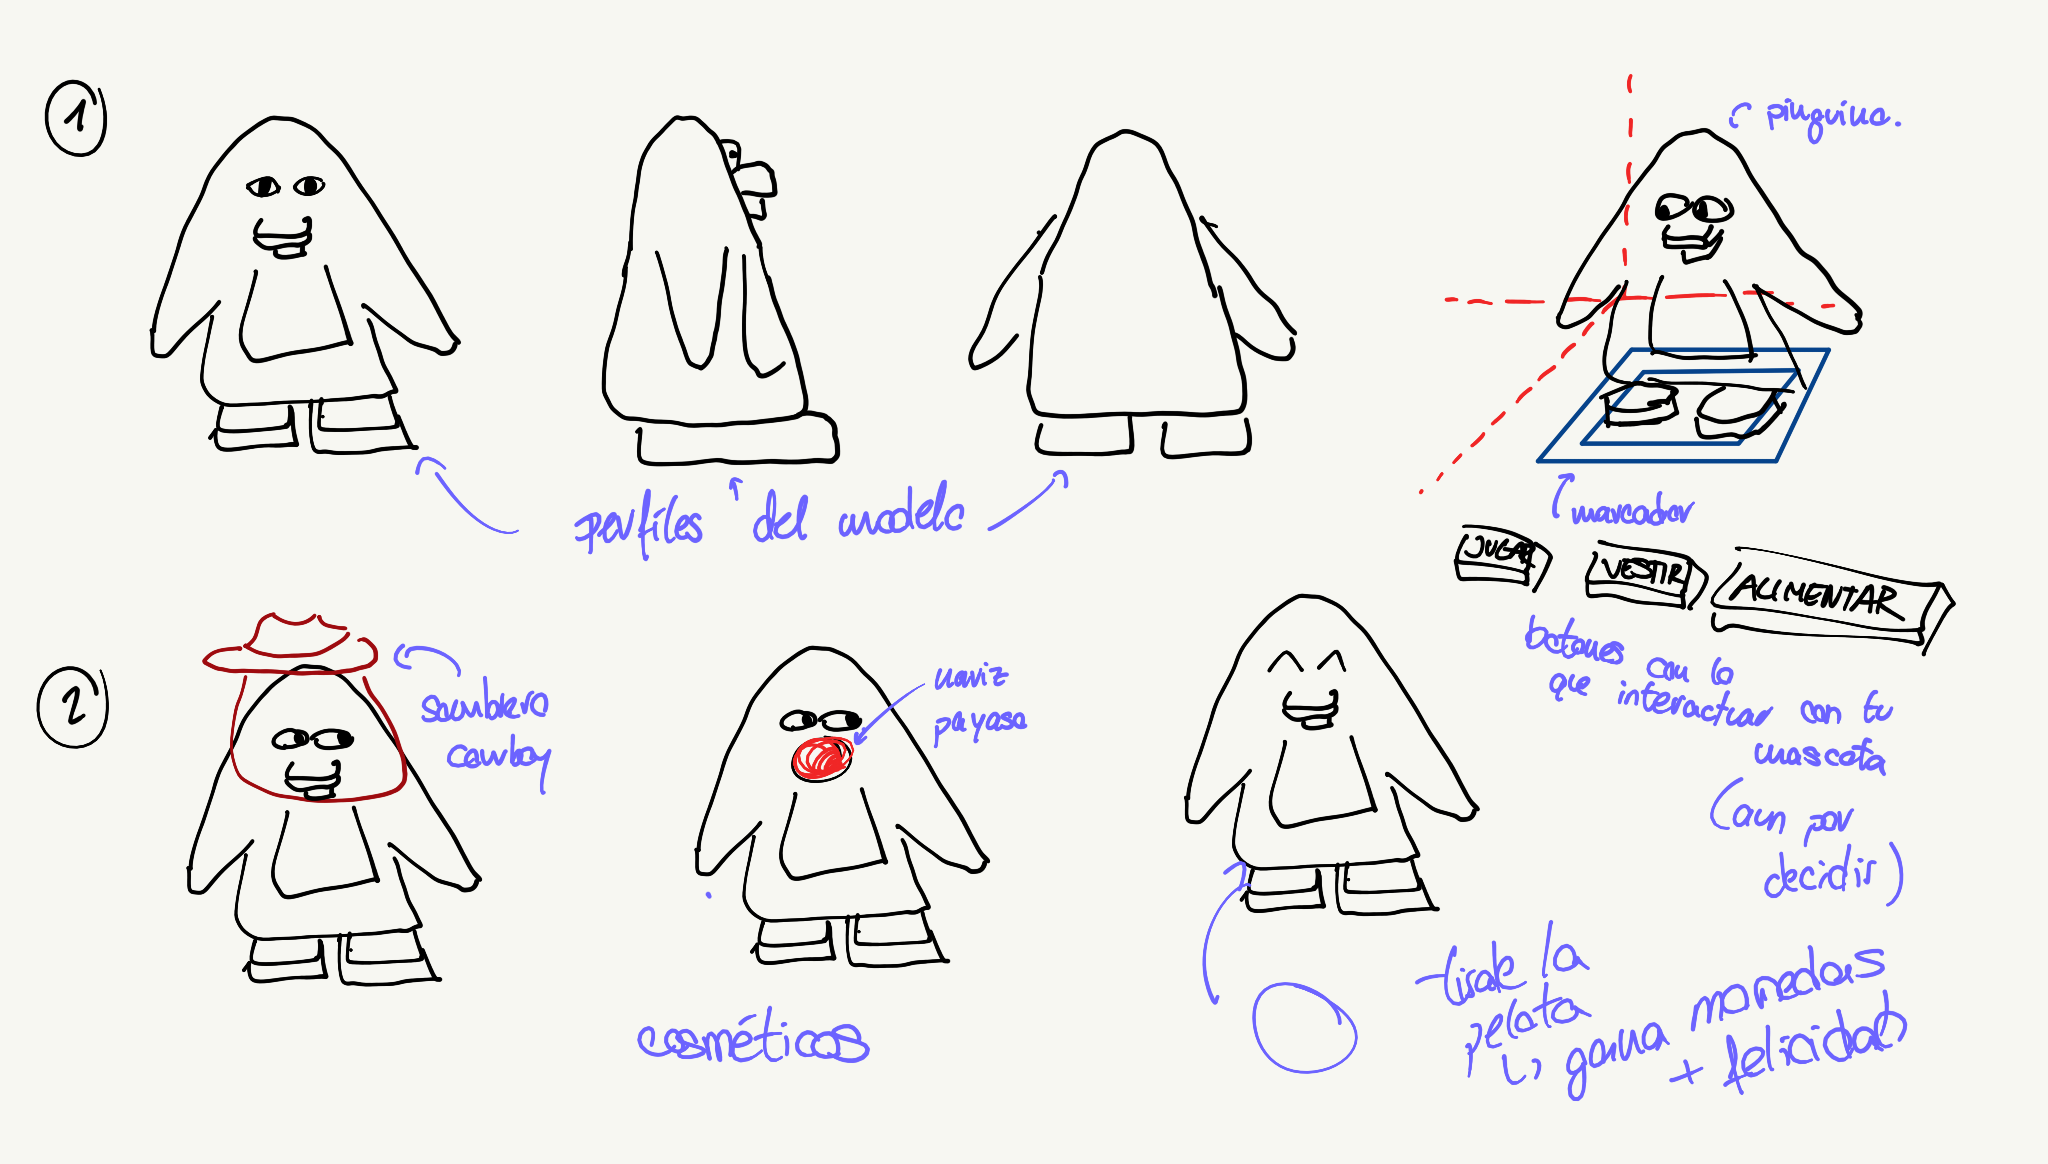
\includegraphics[width=0.8\textwidth]{./images/Boceto1.png}
	\label{fig:boceto1}
\end{figure}

\begin{figure}[htbp]
	\centering
	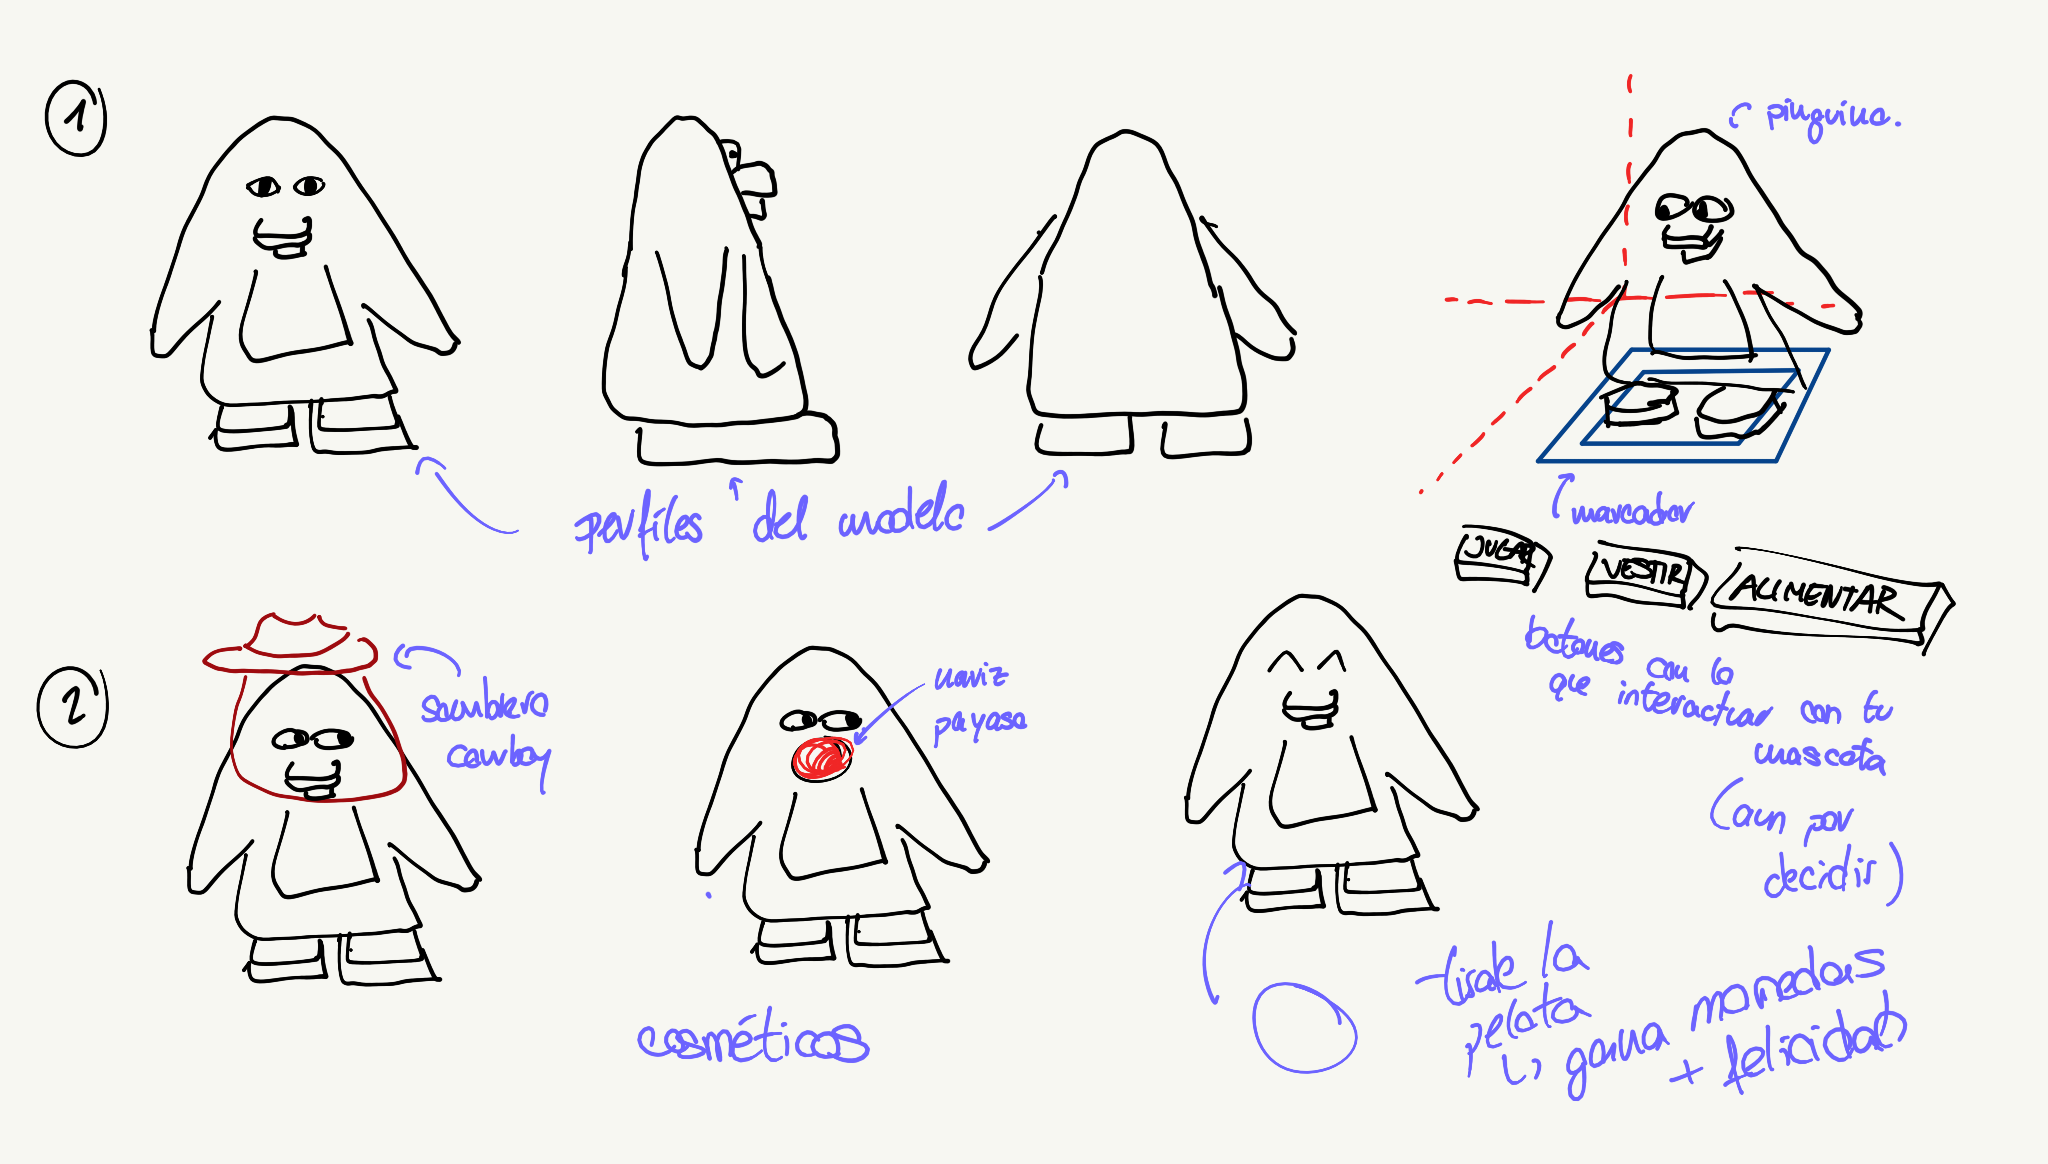
\includegraphics[width=0.8\textwidth]{./images/Boceto1.png}
	\label{fig:boceto2}
\end{figure}




  
  
  
\pagebreak



\clearpage
\end{document}